\newcommand{\GO}[1]{\ensuremath{O(#1)}\xspace}
\newcommand{\SO}[1]{\ensuremath{O\tilde\ (#1)}\xspace}
\newcommand{\vect}[1]{\ensuremath{\mathbf{#1}}\xspace}
\newcommand{\mat}[1]{\ensuremath{\mathbf{#1}}\xspace}
%%%%%%%%%%%%%%%%%%%%%%%%%%%%%%%%%%%%%%%%%%%%%%%%%%%%%ùù
%%%%%%%%%%%%%%%%%%%%%%%%%%%%%%%%%%%%%%%%%%%%%%%%%%%%%ùù
\section{Algorithmic aspect}

Solving exactly over the field of rational numbers, requires a careful attention to the size of the numbers being
manipulated. Indeed, rational numbers are represented by a pair of multiprecision integers, a numerator and
denominator. Applying the standard direct methods designed for solving approximately systems with floating point
rational numbers would lead to a blowup in the bitsize of the coefficients, and result in overwelming computation
overheads, with time complexities often not even polynomial.

In a series of algorithmic innovations, summarized in Table~\ref{tab:complexities}, the time complexity for solving exactly a linear system over the rationals has
been reduced to $\SO{n^3}$ or $\SO{n^\omega}$ which is asymptotically as fast as the complexity for solving
approximately using floating point numbers.

First, the use of rational reconstruction makes it possible to recover the rational solution from the solution of the same
system projected intoa large enough finite field.
This approach avoids the  swell in the bitsize of the intermediate computations and compute with the arithemtic precision of the output for a total cost of $\GO{n^5}$.
Then, using  multi-modular representation and the Chinese Remainder Theorem, reduces this cost  to $\SO{n^4}$.
This cost, corresponding to the arithmetic complexity of Gaussian elimination multiplied by the bitsize of the output,
is a sub-optimal. By better balancing the computation load between numerous arithmetic operation on small bitsize and
few operations on large bitsize, one can hope to further reduce this complexity. This is achieved by $p$-adic lifting
techniques~\cite{Dix82}, reaching a $\SO{n^3}$ time complexity. Improving the complexity for this problem is still a
very active topic: it was then improved by~\cite{Sto05} to $\SO{n^\omega}$ using a randomization, and the same
complexity can now been reached deterministically since this year~\cite{BLS19}.



\begin{table}[htb]
\begin{tabular}{lc}
  \toprule
  Method  & Bit complexity \\
  \midrule
  Gauss over $\mathbb{Q}$ & $2^{\GO{n}}$ \\
  Gauss $\mod \text{bound}(sol)$ & $\GO{n^5}$\\
  CRT $\times$ Gauss $\mod p$ & $\SO{n^4}, \SO{n^\omega+1}$\\
  $p$-adic lifting & $\SO{n^3}, \SO{n^\omega}$\\
  \bottomrule
\end{tabular}
\caption{Brief overview of algorithmic innovations for solving linear systems over the rationals}\label{tab:complexities}
\end{table}

While $p$-adic lifting techniques achieve the best complexity for sequential computations, they are unfortunately very
iterative in their structure, and therefore harder to parallelize at a large scale. On the contrary, Chinese remainder
based methods offer an embarrassingly parallel structure, but cost a factor of $n$ more. We have therefore chosen to
explore both approaches which will be described in the following subsections.
%%%%%%%%%%%%%%%%%%%%%%%%%%%%%%%%%%%%%%%%%%%%%%%%%%%%%ùù
\subsection{The Chinese remainder approach}

We recall here the principle of the Chinese Remainder based rational solver.
\begin{algorithm}
  \caption{Chinese Remainder based rational solver}
  \begin{algorithmic}[1]
    \Require{$\mat{A}\in \mathbb{Z}^{n\times n},\vect{b}\in\mathbb{Z}^n$}
    \Ensure{$\vect{x}$ such that $\mat{A}\vect{x}=\vect{b}$}
    \State $N,D \leftarrow \text{SolutionBounds}(\mat{A},b)$
    \State Pick $\ell$ primes $p_1,\dots, p_\ell$ such that $\prod_{i=1}^\ell p_i \geq 2ND$
    \For{$i\leftarrow 1\dots \ell$}
    \State $\mat{A}^{(i)} \leftarrow \mat{A}\mod p_i$
    \State $\vect{b}^{(i)} \leftarrow \vect{b}\mod p_i$
    \State $\vect{x}^{(i)} \leftarrow (\mat{A}^{(i)})^{-1} \vect{b}^{(i)} \mod p_i$
    \EndFor
  \State $y \leftarrow \texttt{ChineseRemainder}(\vect{y}^{(1)},p_1,\dots, \vect{y}^{(\ell)},p_\ell)$
  \State $\vect{x},d\leftarrow \texttt{VectorRationalReconstruction(\vect{y})}$
  \State \Return $\vect{x}/d$
\end{algorithmic}
\end{algorithm}


%%%%%%%%%%%%%%%%%%%%%%%%%%%%%%%%%%%%%%%%%%%%%%%%%%%%%ùù
\subsection{The $p$-adic lifting approach}

\begin{algorithm}
  \caption{$p$-adic lifting based rational solver}
  \begin{algorithmic}[1]
    \Require{$\mat{A}\in \mathbb{Z}^{n\times n},\vect{b}\in\mathbb{Z}^n$}
    \Ensure{$\vect{x}$ such that $\mat{A}\vect{x}=\vect{b}$}
    \State $N,D \leftarrow \text{SolutionBounds}(\mat{A},b)$
    \State Pick a  primes $p$. Let $k$ such that $p^k \geq 2ND$
    \State $\mat{B}\leftarrow A^{-1} \mod p$
    \State $\vet{r}\leftarrow \vect{b}$
    \For{$i\leftarrow 0\dots k$}
    \State $\vect{c}^{(i)}  \leftarrow \mat{B} \vect{r} \mod p_i$
    \State $\vet{r} \leftarrow  \frac{\vect{r} - \mat{A}\vect{x_i}}{p}$
    \EndFor
    \State $\vect{y} \leftarrow \sum_{i=0}^{k-1} \vect{c}^{(i)} p^i$
    \State $\vect{x},d\leftarrow \texttt{VectorRationalReconstruction(\vect{y})}$
  \State \Return $\vect{x}/d$
\end{algorithmic}
\end{algorithm}

%%%%%%%%%%%%%%%%%%%%%%%%%%%%%%%%%%%%%%%%%%%%%%%%%%%%%ùù
%%%%%%%%%%%%%%%%%%%%%%%%%%%%%%%%%%%%%%%%%%%%%%%%%%%%%ùù
\section{High performance parallelization}

The implementations referred to for this deliverable are made in the \Linbox library.


%%%%%%%%%%%%%%%%%%%%%%%%%%%%%%%%%%%%%%%%%%%%%%%%%%%%%ùù
\subsection{MPI based Chinese remainder algorithm}
\begin{figure}[htb]
\begin{center}
  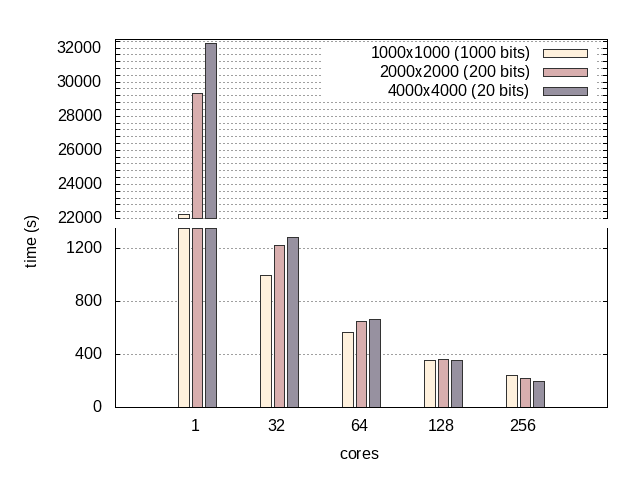
\includegraphics[width=.7\textwidth]{nodes_histogram}
\end{center}
\caption{MPI-Chinese Remainder based rational solver.}\label{fig:mpi_histo}
\end{figure}
%%%%%%%%%%%%%%%%%%%%%%%%%%%%%%%%%%%%%%%%%%%%%%%%%%%%%ùù
\subsection{A multicore $p$-adic lifting}

Adapted from and improving on \cite{ChSt05}.

%%%%%%%%%%%%%%%%%%%%%%%%%%%%%%%%%%%%%%%%%%%%%%%%%%%%%ùù
\subsection{GPU enabled libraries}


\bibliographystyle{plainnat}
\bibliography{D5.14}

%% LaTeX-Master: report.tex
%% mode: latex

